\documentclass[a4paper]{article}

\usepackage[spanish]{babel}
\usepackage[utf8]{inputenc}
\usepackage{amsmath}
\usepackage{graphicx}
\usepackage[colorinlistoftodos]{todonotes}





\title{Segmentaci'on de retornos de la bolsa de valores de S $\&$ P 500}

\author{Mar\'ia Arg\'aez Autor\corref{cor1}\fnref{label2}}
\date{\today}

\begin{document}

\begin{abstract}
Este art\'iculo presenta un an\'alisis de datos que involucra un an\'alisis exploratorio de datos desde medidas descriptivas hasta segmentaci\'on de datos utilizando algoritmos de aprendizaje autom\'atico no supervisado como el K-means. 
\end{abstract}


\section{Introducci\'on}

El an\'alisis exploratorio de datos brinda una idea general del comportamiento de los datos estad\'isticamente, en donde se utilizan medidas centrales y de dispersi\'on como la media, la mediana, desviaci\'on estandar, varianza y rango.

% https://www.mjandrews.org/book/ddsr/assets/chapter_05_exploratory.pdf

La agrupaci\'on en cl\'usteres o segmentaci\'on, es una t\'ecnica computacional que divide las muestras de conjunto de datos en grupos. Una agrupaci\'on exitosa da como resultado grupos que contienen puntos que est\'an relacionados entre s\'i. Si esas relaciones son significativas generalmente requiere verificaci\'on humana.
% https://livebook.manning.com/book/classic-computer-science-problems-in-python/chapter-6/1

 

[1] 

Una forma en que las organizaciones pueden recaudar fondos para expandir su negocio o pagar la deuda es cotizando en bolsa y emitiendo acciones que luego se negocian en los mercados secundarios, también conocidos como bolsas de valores. La empresa ofrece acciones en lugar de pedir prestado capital en forma de efectivo, esto le permite a la empresa evitar sus posibilidades de incurrir en pérdidas, deudas y pagar tasas de interés. De igual manera, para los accionistas, es posible obtener beneficios y ganar dinero. Estos accionistas, o inversionistas, pueden obtener ganancias ya sea de las empresas cuyas acciones pagan dividendos regulares o vendiendo sus acciones en el mercado cuando las acciones de la empresa alcanzan una tasa más alta que la que se compró. {1} 

Los mercados de capital accionario, también conocidos en inglés como stocks o shares, funcionan como una plataforma de emisión y negociación de acciones de sociedades cotizadas. 

Las acciones, o participaciones, revisan la posesión fragmentaria en una organización, recurso o valor, y de esta manera, que el mercado de valores funciona como una plataforma para los patrocinadores financieros donde pueden comprar y vender recursos u ofertas invertibles tomando en cuenta una gran responsabilidad ya que se pone en juego dinero. Las personas que participan en dicho intercambio de acciones y activos se denominan participantes del mercado, entre los cuales es posible mencionar participantes minoristas nacionales, NRI y ciudadanos de la India en el extranjero (OCI), instituciones nacionales, empresas de gestión de activos nacionales (AMC) o inversores extranjeros.´{1} 

Un instrumento financiero es un contrato de activos negociables como acciones, bonos, letras, divisas, swaps, futuros y opciones, que otorga el derecho a poseer una entidad en parte o en su totalidad o a reclamar los activos de la entidad. Los activos financieros son derechos sobre los ingresos producidos por los activos reales (por ejemplo, la venta de granos de cacao, el alquiler de un edificio, la prestación de un servicio) y entre los instrumentos financieros podemos mencionar capital, bolsas de valores, índice bursátil, comercio de acciones, bonos, derivados, divisas y materias primas. [2] 

Por lo tanto, predecir el valor de mercado de las acciones es de gran interés para quienes participan en el mercado de valores. 

Una de las aplicaciones del aprendizaje automatico es en finanzas, especificamente en aquellos  algoritmos y técnica que se centran en la predicción de acciones. La predicción del mercado de valores es el intento que se hace para pronosticar o predecir el próximo valor de la acción, el sector del mercado o incluso todo el mercado y es un área que ha llamado la atención de muchas personas, incluidas no solo empresas, sino también comerciantes, participantes del mercado, analistas de datos e incluso ingenieros informáticos que trabajan en el dominio del aprendizaje automático (ML) y la inteligencia artificial (AI), etc.  

En los mercados financieros, el aprendizaje automático (ML) se ha convertido en una poderosa herramienta analítica utilizada para ayudar y administrar la inversión de manera eficiente. ML se ha utilizado ampliamente en el sector financiero para proporcionar un nuevo mecanismo que puede ayudar a los inversores a tomar mejores decisiones tanto en inversión como en gestión para lograr un mejor rendimiento de su mercado de calcetines de inversión en valores. Por lo tanto, los inversores deben comprender la naturaleza de las acciones individuales y los factores de dependencia que afectan a los precios de las acciones para aumentar sus posibilidades de lograr mayores rendimientos. [2]  

La inversión de fondos en el mercado está sujeta a varios riesgos de mercado, ya que el valor de las acciones de la empresa depende en gran medida de las ganancias y el desempeño de la organización en el mercado y, por lo tanto, puede variar debido a varios factores, como políticas gubernamentales, indicadores microeconómicos. , demanda y oferta, etc. Estas variaciones en el mercado se estudian para desarrollar software y programas utilizando diversas técnicas como ML, Deep Learning, Neural Networks, AI, etc. 

Dichos sistemas y software pueden permitir al inversor anticipar adecuadamente la situación de la empresa, sobre la base de datos pasados y presentes, la condición actual del mercado, etc. y darle una dirección para tomar decisiones para que no pierda. su valioso dinero y obtener los máximos beneficios. Sin embargo, la predicción de precios basada en algunos factores sería fácil, pero el resultado podría ser inexacto porque algunos factores excluidos también pueden ser importantes para explicar el movimiento de los precios de las acciones. Los precios de las acciones individuales pueden verse afectados por varios factores, como los sentimientos y las emociones humanas. 

\section{Marco Te\'orico}
INTRODUCCIÓN 

[1] 

Una forma en que las organizaciones pueden recaudar fondos para expandir su negocio o pagar la deuda es cotizando en bolsa y emitiendo acciones que luego se negocian en los mercados secundarios, también conocidos como bolsas de valores. La empresa ofrece acciones en lugar de pedir prestado capital en forma de efectivo, esto le permite a la empresa evitar sus posibilidades de incurrir en pérdidas, deudas y pagar tasas de interés. De igual manera, para los accionistas, es posible obtener beneficios y ganar dinero. Estos accionistas, o inversionistas, pueden obtener ganancias ya sea de las empresas cuyas acciones pagan dividendos regulares o vendiendo sus acciones en el mercado cuando las acciones de la empresa alcanzan una tasa más alta que la que se compró. {1} 

Los mercados de capital accionario, también conocidos en inglés como stocks o shares, funcionan como una plataforma de emisión y negociación de acciones de sociedades cotizadas. 

Las acciones, o participaciones, revisan la posesión fragmentaria en una organización, recurso o valor, y de esta manera, que el mercado de valores funciona como una plataforma para los patrocinadores financieros donde pueden comprar y vender recursos u ofertas invertibles tomando en cuenta una gran responsabilidad ya que se pone en juego dinero. Las personas que participan en dicho intercambio de acciones y activos se denominan participantes del mercado, entre los cuales es posible mencionar participantes minoristas nacionales, NRI y ciudadanos de la India en el extranjero (OCI), instituciones nacionales, empresas de gestión de activos nacionales (AMC) o inversores extranjeros.´{1} 

Un instrumento financiero es un contrato de activos negociables como acciones, bonos, letras, divisas, swaps, futuros y opciones, que otorga el derecho a poseer una entidad en parte o en su totalidad o a reclamar los activos de la entidad. Los activos financieros son derechos sobre los ingresos producidos por los activos reales (por ejemplo, la venta de granos de cacao, el alquiler de un edificio, la prestación de un servicio) y entre los instrumentos financieros podemos mencionar capital, bolsas de valores, índice bursátil, comercio de acciones, bonos, derivados, divisas y materias primas. [2] 

Por lo tanto, predecir el valor de mercado de las acciones es de gran interés para quienes participan en el mercado de valores. 

Una de las aplicaciones del aprendizaje automatico es en finanzas, especificamente en aquellos  algoritmos y técnica que se centran en la predicción de acciones. La predicción del mercado de valores es el intento que se hace para pronosticar o predecir el próximo valor de la acción, el sector del mercado o incluso todo el mercado y es un área que ha llamado la atención de muchas personas, incluidas no solo empresas, sino también comerciantes, participantes del mercado, analistas de datos e incluso ingenieros informáticos que trabajan en el dominio del aprendizaje automático (ML) y la inteligencia artificial (AI), etc.  

En los mercados financieros, el aprendizaje automático (ML) se ha convertido en una poderosa herramienta analítica utilizada para ayudar y administrar la inversión de manera eficiente. ML se ha utilizado ampliamente en el sector financiero para proporcionar un nuevo mecanismo que puede ayudar a los inversores a tomar mejores decisiones tanto en inversión como en gestión para lograr un mejor rendimiento de su mercado de calcetines de inversión en valores. Por lo tanto, los inversores deben comprender la naturaleza de las acciones individuales y los factores de dependencia que afectan a los precios de las acciones para aumentar sus posibilidades de lograr mayores rendimientos. [2]  

La inversión de fondos en el mercado está sujeta a varios riesgos de mercado, ya que el valor de las acciones de la empresa depende en gran medida de las ganancias y el desempeño de la organización en el mercado y, por lo tanto, puede variar debido a varios factores, como políticas gubernamentales, indicadores microeconómicos. , demanda y oferta, etc. Estas variaciones en el mercado se estudian para desarrollar software y programas utilizando diversas técnicas como ML, Deep Learning, Neural Networks, AI, etc. 

Dichos sistemas y software pueden permitir al inversor anticipar adecuadamente la situación de la empresa, sobre la base de datos pasados y presentes, la condición actual del mercado, etc. y darle una dirección para tomar decisiones para que no pierda. su valioso dinero y obtener los máximos beneficios. Sin embargo, la predicción de precios basada en algunos factores sería fácil, pero el resultado podría ser inexacto porque algunos factores excluidos también pueden ser importantes para explicar el movimiento de los precios de las acciones. Los precios de las acciones individuales pueden verse afectados por varios factores, como los sentimientos y las emociones humanas. 

\section{Material y m\'etodos}
Los datos que se utilizaron fueron 5 a\~{n}os de historia diaria de la bolsa de valores llamada "S \& P 500", la cual cuenta con valores como el 'Open '  (Apertura), ' Close' (cierre), 'High' (alto), 'Low' (bajo). Estas medidas de la serie de tiempo con medidas  refleja el precio m\'inimo y m\'aximo de la bolsa asi como el precio con el que abrio y cerro. 

Se calcularon los retornos con la serie de tiempo del cierre de la acción, lo cu\'al es la divisón del valor anterior del cierre entre el actual. Además se categorizaron los retornos en positivos o negativos. El escenario ideal seria aquel en el que todos los retornos son positivo, por el contrario, el peor escenario seria en el que todos los retornos son negativos, en si, una acción de la bolsa de valores debe tener más retornos positivos que negativos para que tenga un buen retorno de inversión para toda aquella persona que desee invertir en ella. Por tanto, también se categorizaron los retornos en 1 si el retorno era positivo o negativo. 

Se conoce que existen diversos tipos bolsa de valores, en este caso "S $\&$ P 500", son las siglas en ingl\'es de "Standard and Poor's 500", el cu\'al es un \'indice burs\'atil que rastrea el rendimiento de las acciones de 500 grandes empresas que cotizan en las bolsas de valores de los Estados Unidos y representa uno de los \'indices burs\'atiles m\'as seguidos.

Para este an\'alisis se utilizo el software libre de python y librerias de sklearn donde se utiliz\'o el algoritmo de K - means.



\section{Experimento}
Se utiliz\'o un $ K =2$ ya que de antemano se sabia que los retornos se clasifican en dos grupos, positivos y negativos.  De tal manera, que utilizando el algoritmo se segmentaron las clases como se observa en la imagen 1.

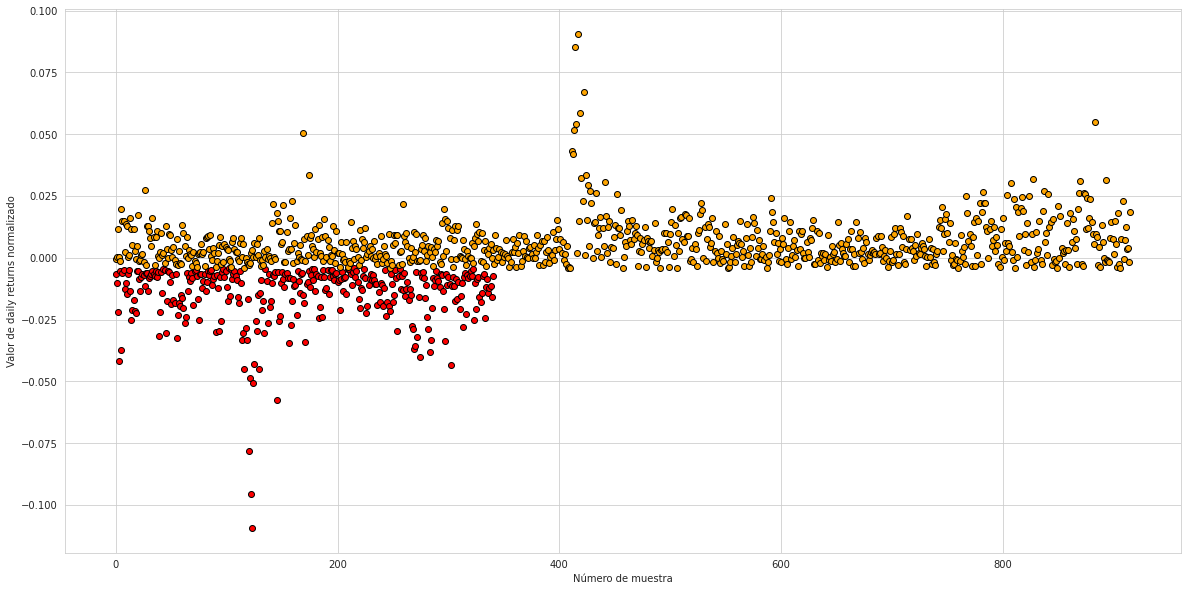
\includegraphics[scale=0.2]{segmentacion.png}

\section{C\'alculos}

El pseudoc\'odigo que se plantea en el algoritmo de k-means es el siguiente.

1. Primero se declaran los inputs como la muestra $D$ y el número de cl\'usters que se quiere, $k$.

2. Despu\'es se elige para cada muestra, dato o punto un cluster como su centroide inicial y despu\'es se calcula la distancias con cada punto con cada uno de los centroides y se asigna a cada punto el centroide con menor distancia. 

3. El paso 2 se repite hasta que las distancias ya no cambian , es decir , convergieron a un punto en el que cada punto ya tiene a su centroide m\'as cercano. 


\section{Resultados}

 Se observa que para dos clusters, la mayoria de los muestras son repartieron en retornos positivos y negativos en el cual corresponde a los puntos color amarillo y rojo respectivamente de la imagen 1. 

\section{Conclusi\'on}

Se concluye que el algoritmo de Kmeans realiz\'o una segmentaci\'on acorde a lo que hab\'ia planteado, agrupando a los retornos positivos y negativos en dos clusters.





\end{document}